\documentclass[12pt,a4paper]{report}

\usepackage[utf8]{inputenc}
\usepackage[T1]{fontenc}
\usepackage[english,provide=*]{babel}
\babelprovide[import,main]{czech}
\usepackage[a4paper,left=2.5cm,right=2.5cm,top=3cm,bottom=3cm]{geometry}
\usepackage{setspace}
\usepackage{hyperref}
\usepackage{booktabs}
\usepackage{tabularx}
\usepackage{array}
\usepackage{enumitem}
\usepackage{fancyhdr}
\usepackage{titlesec}
\usepackage{needspace}
\usepackage{etoolbox}
\usepackage{amsmath}
\usepackage{amssymb}
\usepackage{longtable}
\usepackage{caption}
\usepackage{tikz}
\usetikzlibrary{positioning,arrows.meta,shapes.geometric,fit}

\raggedbottom
\setstretch{1.25}
\emergencystretch=2em
\setlength{\headheight}{15pt}
\setlist[itemize]{leftmargin=1.6em,topsep=0.35\baselineskip,itemsep=0.2\baselineskip,parsep=0pt,partopsep=0pt}
\setlist[enumerate]{leftmargin=1.9em,topsep=0.35\baselineskip,itemsep=0.2\baselineskip,parsep=0pt,partopsep=0pt}
\clubpenalty=10000
\widowpenalty=10000
\displaywidowpenalty=10000

\hypersetup{
  colorlinks=true,
  linkcolor=blue,
  urlcolor=blue,
  pdftitle={SkillHub -- Oficiální dokumentace maturitního projektu},
  pdfauthor={Lukáš Levinský},
  pdfsubject={Maturitní projekt},
  pdfkeywords={SkillHub, dovednosti, e-learning, doporučování, maturitní projekt}
}

\addto\captionsczech{%
  \renewcommand{\figurename}{Obr.}%
  \renewcommand{\tablename}{Tab.}%
}

\pagestyle{fancy}
\fancyhf{}
\fancyhead[L]{SkillHub -- Dokumentace maturitního projektu}
\fancyhead[R]{\thepage}

\titleformat{\chapter}{\normalfont\LARGE\bfseries}{\thechapter.}{0.7em}{}
\titlespacing*{\chapter}{0pt}{0.5\baselineskip}{1.1\baselineskip}
\titlespacing*{\section}{0pt}{0.9\baselineskip}{0.45\baselineskip}
\titlespacing*{\subsection}{0pt}{0.7\baselineskip}{0.35\baselineskip}
\pretocmd{\section}{\Needspace{10\baselineskip}}{}{}
\pretocmd{\subsection}{\Needspace{8\baselineskip}}{}{}

\newcommand{\studyField}{Informační technologie}
\newcommand{\className}{4.B}

\begin{document}
\selectlanguage{czech}
\hypersetup{pageanchor=false}
\pagenumbering{gobble}

\begin{titlepage}
\centering

{\large DELTA -- Střední škola informatiky a ekonomie, s.r.o.\\
Ke Kamenci 151, Pardubice\par}
\vspace{1.8cm}

{\Huge \textbf{SkillHub}\par}
\vspace{0.3cm}
{\Large Webová platforma pro plánování a rozvoj dovedností\par}
\vspace{1.8cm}

\begin{tabular}{>{\bfseries}l l}
Autor: & Lukáš Levinský \\
Studijní obor: & \studyField \\
Třída: & \className \\
Vedoucí projektu: & Ing. Veronika Hořeňovská \\
Školní rok: & 2025/2026 \\
Datum: & \today \\
\end{tabular}

\end{titlepage}

\clearpage
\thispagestyle{empty}
\begin{center}
\textbf{Zadání maturitního projektu}
\end{center}
\vspace{1cm}
Do finální tištěné verze se na toto místo vkládá schválený a podepsaný list \textit{Zadání maturitního projektu}. V repozitáři je k dispozici pouze obecný dokument s pokyny pro zpracování, nikoli individuální zadání autora.

\clearpage
\thispagestyle{empty}
Prohlašuji, že jsem maturitní projekt vypracoval samostatně, výhradně s použitím uvedené literatury a dalších citovaných zdrojů.

\vspace{1.6cm}
V Pardubicích dne \dotfill

\vspace{1.6cm}
Podpis: \dotfill

\clearpage
\thispagestyle{empty}
Upřímně děkuji vedoucí projektu Ing. Veronice Hořeňovské za odborné vedení, průběžné konzultace a připomínky při zpracování maturitního projektu. Poděkování patří také všem, kteří pomohli s testováním, odbornou zpětnou vazbou a průběžnou revizí návrhu.

\clearpage
\chapter*{Resumé}
\addcontentsline{toc}{chapter}{Resumé}
Tato dokumentace popisuje maturitní projekt SkillHub, tedy webovou platformu zaměřenou na plánování a rozvoj dovedností. Projekt reaguje na problém běžných e-learningových služeb, které obvykle pracují hlavně s katalogem kurzů, ale už méně s dlouhodobým rozvojem konkrétních kompetencí. Navržené řešení proto staví do centra datového modelu dovednostní profil uživatele, na který jsou navázány kurzy, testy, doporučování i motivační prvky. Cílem systému je pomoci uživateli určit, co se učit, proč je to pro něj vhodné a jak ověřit dosažený pokrok.

Technická realizace využívá samostatný frontend, backendové REST API, relační databázi, cache a oddělenou AI službu pro sémantické doporučování. Dokumentace shrnuje východiska projektu, hlavní návrhová rozhodnutí, architekturu systému, důležité algoritmy, dosažené výsledky a limity dalšího rozvoje.

\vspace{0.7cm}
\noindent\textbf{Klíčová slova:} SkillHub, dovednosti, e-learning, doporučovací systém, gamifikace, REST API, architektura systému, maturitní projekt.

\clearpage
\chapter*{Summary}
\addcontentsline{toc}{chapter}{Summary}
This documentation describes the SkillHub graduation project, a web platform focused on skill planning and long-term skill development. The project addresses a common limitation of standard e-learning platforms: they usually organize content around courses, but they do not provide strong support for structured growth in specific competencies. SkillHub therefore places the user's skill profile at the center of the system and connects it with courses, tests, recommendations, and motivational features. The goal is to help the user decide what to learn, why it is relevant, and how to verify real progress.

The technical solution consists of a standalone frontend, a REST backend API, a relational database, a cache layer, and a separate AI service for semantic recommendations. The documentation summarizes the project background, main design decisions, system architecture, key algorithms, achieved results, and current limitations.

\vspace{0.7cm}
\noindent\textbf{Keywords:} SkillHub, skills, e-learning, recommendation system, gamification, REST API, system architecture, graduation project.

\clearpage
\begingroup
\small
\setstretch{1.05}
\tableofcontents
\endgroup
\clearpage
\hypersetup{pageanchor=true}
\pagenumbering{arabic}
\setcounter{page}{8}

\chapter*{Úvod}
\addcontentsline{toc}{chapter}{Úvod}
Online vzdělávání nabízí velké množství obsahu, ale uživateli často neposkytuje dostatečnou oporu při plánování vlastního rozvoje. Typická platforma odpovídá především na otázku, jaké kurzy jsou dostupné. Méně často však řeší, jaké dovednosti si má uživatel budovat, jak má postupovat po dokončení jednoho kurzu a jak může ověřit, že se skutečně zlepšil. Tento problém je dlouhodobě patrný jak u komerčních vzdělávacích platforem, tak u menších interních systémů, které se obvykle soustředí na distribuci obsahu spíše než na řízení kompetenčního růstu.

Maturitní projekt SkillHub vznikl jako pokus navrhnout systém, který bude místo katalogového přístupu pracovat s dovednostmi jako s hlavní doménovou entitou. Inspirací byly obecné principy moderních webových aplikací, doporučovacích systémů a práce se strukturovaným uživatelským profilem \cite{next,react,express,reimers}. Projekt má sloužit jako funkční ukázka toho, že i ve školním rozsahu lze vytvořit systém, který propojuje evidenci dovedností, výběr studijního obsahu, testování a průběžnou motivaci.

Cílem práce je navrhnout a implementovat webovou aplikaci, která:
\begin{itemize}
  \item umožňuje evidovat dovednostní profil uživatele,
  \item doporučuje kurzy a další obsah podle aktuálního stavu profilu,
  \item podporuje testování a verifikaci úrovně znalostí,
  \item nabízí volitelnou gamifikační vrstvu pro dlouhodobější motivaci,
  \item zůstává přehledná, rozšiřitelná a dobře obhajitelná při obhajobě projektu.
\end{itemize}

\chapter{Teoretická část}
\section{Dovednostně orientovaný přístup}
Základním rozdílem mezi běžnou kurzovou platformou a systémem typu SkillHub je volba hlavní entity. V klasickém katalogu je primárním objektem kurz. Uživatel si vybírá obsah a po jeho dokončení se přesouvá k dalšímu. Dovednostně orientovaný přístup naopak vychází z toho, že výsledkem učení nemá být prosté zhlédnutí nebo absolvování materiálu, ale posun v konkrétní kompetenci. Kurz je tedy pouze prostředkem, nikoliv cílem. Tento způsob uvažování je vhodný pro systémy, které chtějí podporovat dlouhodobější plánování a měřitelný pokrok.

Pro SkillHub z toho plynou tři důležité zásady. Za prvé musí být možné modelovat dovednost, její návaznosti a úroveň zvládnutí. Za druhé musí být studijní obsah propojen s dovednostmi, nikoliv veden izolovaně. Za třetí musí existovat možnost pokrok nejen deklarovat, ale také ověřit.

\section{Doporučovací systémy}
Doporučovací mechanismy mohou být postaveny na pravidlech, na obsahové podobnosti nebo na sémantickém porozumění textu. Pravidlový přístup je stabilní a dobře vysvětlitelný, ale hůře si poradí s různými formulacemi téhož cíle. Obsahový přístup založený na shodě tagů a vlastností je vhodný tam, kde je datový model dobře připraven, ale bývá méně pružný při práci s nejednoznačným vstupem. Sémantické doporučování využívá vektorové reprezentace textu a umožňuje porovnávat významovou podobnost i tehdy, když uživatel použije jiná slova než autor obsahu \cite{reimers,fastapi}.

V projektu SkillHub je vhodné využít hybridní přístup. Pravidla zajišťují stabilitu a transparentnost, zatímco sémantická vrstva zvyšuje přesnost u textových vstupů typu „chci začít s frontendem“ nebo „potřebuji zlepšit JavaScript“. Takové formulace se nemusí přesně shodovat s názvy uložených dovedností nebo kurzů, ale významově k nim mají blízko.

\section{Současný stav a konkurence}
Na trhu existuje řada zavedených platforem, které řeší online vzdělávání ve velkém měřítku. Typickými zástupci jsou Udemy, Coursera nebo LinkedIn Learning. Jejich silnou stránkou je především rozsáhlý katalog a kvalitní distribuční zázemí. Slabší bývá transparentní práce s osobním skill profilem, vysvětlitelnost doporučení a možnost přizpůsobit celý systém konkrétnímu školnímu nebo internímu použití.

Srovnání hlavních principů shrnuje tab. \ref{tab:comparison}. SkillHub není navržen jako náhrada velkých globálních platforem, ale jako specializovaný systém pro řízený rozvoj dovedností.

\begin{table}[ht]
\centering
\caption{Srovnání SkillHub s typickou kurzovou platformou}
\label{tab:comparison}
\begin{tabularx}{\textwidth}{>{\raggedright\arraybackslash}p{4.2cm} >{\raggedright\arraybackslash}X >{\raggedright\arraybackslash}X}
\toprule
Kritérium & SkillHub & Typická kurzová platforma \\
\midrule
Primární objekt systému & dovednost a rozvoj uživatele & kurz nebo program \\
Osobní skill profil & přímá součást datového modelu & často jen nepřímé sledování \\
Doporučování & kombinace pravidel a sémantiky & zpravidla interní black-box \\
Ověření pokroku & testy a verifikace úrovně & nejčastěji jen dokončení kurzu \\
Možnost úprav systému & vysoká, otevřený vlastní projekt & nízká, uzavřená služba \\
Social funkce & dobrovolné zapnutí uživatelem & zpravidla pevná součást produktu \\
\bottomrule
\end{tabularx}
\end{table}

\section{Bezpečnost a formální kvalita}
Protože jde o softwarový projekt s autentizací, API a uživatelskými daty, musí návrh respektovat i bezpečnostní principy. Důležité je oddělení identity od doménového modelu, validace všech vstupů, kontrola oprávnění a důsledná práce s rolí uživatele. Pro obecný bezpečnostní rámec lze vycházet z doporučení OWASP \cite{owasp}. Stejně důležitá je i formální kvalita dokumentace: použití zdrojů musí být citováno, tabulky a obrázky musí být označeny a text má být věcný, nikoliv marketingový. Tento požadavek vyplývá přímo ze školních pokynů a ovlivnil i zkrácenou podobu této dokumentace.

\chapter{Metodika a vlastní řešení}
\section{Postup práce}
Řešení projektu probíhalo iterativně. Nejprve byl vymezen problém a stanoven rozsah projektu. Následovala analýza domény, návrh datového modelu a architektury, implementace základních modulů a průběžné ověřování funkčnosti. Součástí práce bylo i průběžné porovnávání návrhu s původním cílem projektu, aby řešení neztratilo směr a nerozšířilo se o prvky, které by byly technicky zajímavé, ale pro samotný cíl nepodstatné.

Prakticky byl postup rozdělen do těchto kroků:
\begin{enumerate}
  \item definice hlavních uživatelských scénářů,
  \item návrh datového modelu a architektury systému,
  \item implementace autentizace, profilu a práce s dovednostmi,
  \item doplnění kurzů, testů a doporučovací vrstvy,
  \item rozšíření o sociální a gamifikační prvky,
  \item testování a průběžná revize dokumentace.
\end{enumerate}

\section{Architektura systému}
Systém je rozdělen do tří hlavních částí: frontend, backend a AI služba. Frontend zajišťuje uživatelské rozhraní a komunikaci s API. Backend je odpovědný za business logiku, validaci, autorizaci a práci s databází. AI služba zajišťuje sémantické výpočty používané při doporučování. Toto rozdělení umožňuje držet hlavní aplikaci přehlednou a současně oddělit výpočetně odlišnou vrstvu s jinými knihovnami a runtime.

Přehled použitých technologií je záměrně zhuštěn do jedné stránky, jak doporučují školní pokyny. Tab. \ref{tab:tech} neobsahuje marketingové popisy nástrojů, ale jen jejich roli a důvod použití.

\begin{table}[ht]
\centering
\caption{Přehled použitých technologií a důvod jejich volby}
\label{tab:tech}
\begin{tabularx}{\textwidth}{>{\raggedright\arraybackslash}p{3.1cm} >{\raggedright\arraybackslash}p{3.2cm} X}
\toprule
Vrstva & Řešení & Důvod volby \\
\midrule
Frontend & Next.js 16, React 19 & moderní základ pro větší webovou aplikaci, dobrá práce s routováním a oddělením veřejných a privátních částí \cite{next,react} \\
Backend & Express 5, TypeScript & přehledná REST architektura bez zbytečné abstrakce, plná kontrola nad middleware vrstvou \cite{express} \\
Datová vrstva & PostgreSQL, Prisma ORM & relační model dobře odpovídá povaze systému a Prisma usnadňuje práci se schématem i typovou bezpečnost \cite{prisma} \\
Autentizace & Supabase Auth & oddělení identity od doménového modelu a omezení rizik vlastní implementace auth \cite{supabase} \\
Cache & Redis & zrychlení často čtených dat a snížení zátěže databáze \cite{redis} \\
AI služba & FastAPI, sentence-transformers & samostatná služba pro sémantickou podobnost bez zavlečení ML závislostí do backendu \cite{fastapi,reimers} \\
\bottomrule
\end{tabularx}
\end{table}

\section{Datový model}
U informačního systému je důležité, aby dokumentace nepopisovala jen obrazovky a použité knihovny, ale i samotná data. V implementaci je datový model definován v souboru \texttt{backend/prisma/schema.prisma}. Základní idea návrhu je jednoduchá: identita uživatele je oddělena od jeho studijního stavu, dovednosti tvoří samostatnou hierarchii a všechny důležité akce systému jsou navázány na několik stabilních entit.

Centrálním modelem je \texttt{User}. Ten uchovává profil, roli, vazbu na region a volitelné social statistiky. Na uživatele je napojen model \texttt{UserSkill}, který reprezentuje vztah mezi konkrétním člověkem a konkrétní dovedností. Do tohoto mezimodelu se ukládá úroveň znalosti, průběžný progres, cílová úroveň a informace o verifikaci. Díky tomu není dovednost vlastností systému obecně, ale vždy vztahem mezi katalogem a konkrétním uživatelem.

Model \texttt{Skill} tvoří katalog dovedností. Obsahuje identifikátor, název, slug, popis, kategorii a vazbu na rodičovskou dovednost. Hierarchická struktura je důležitá proto, aby bylo možné spojovat obecnější oblasti, například ``webový vývoj'', s konkrétnějšími položkami typu ``React'' nebo ``REST API''. Na dovednosti jsou navázány kurzy, testy i verifikační otázky.

Studijní obsah reprezentuje model \texttt{Course}. Ten je s dovednostmi propojen přes vazební tabulku \texttt{CourseSkill}, kde se ukládá také relevance vazby. Testovací část je tvořena entitami \texttt{Test}, \texttt{TestQuestion}, \texttt{TestChoice} a \texttt{TestAttempt}. Gamifikační vrstva je oddělena do modelů \texttt{Quest}, \texttt{QuestCompletion} a \texttt{XPTransaction}. Takové rozdělení zlepšuje čitelnost schématu a zároveň umožňuje rozšiřovat jednotlivé oblasti bez zásahu do ostatních částí systému.

\section{Use Case diagram}
Z pohledu UML je důležité popsat hlavní aktéry systému a činnosti, které systém poskytuje. Přehled nejdůležitějších interakcí ukazuje obr. \ref{fig:usecase}.

\begin{figure}[ht]
\centering
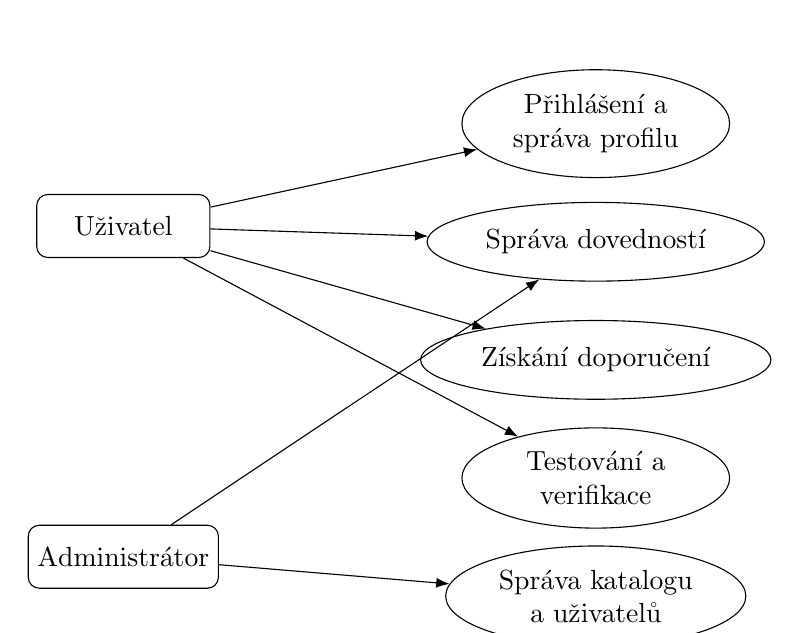
\begin{tikzpicture}[
  actor/.style={draw, rounded corners, minimum width=2.2cm, minimum height=0.8cm, align=center},
  usecase/.style={draw, ellipse, minimum width=3.4cm, minimum height=1cm, align=center},
  >=Latex
]
\node[actor] (user) at (0,0) {Uživatel};
\node[actor] (admin) at (0,-4.2) {Administrátor};

\node[usecase] (auth) at (6,1.3) {Přihlášení a\\správa profilu};
\node[usecase] (skills) at (6,-0.2) {Správa dovedností};
\node[usecase] (recommend) at (6,-1.7) {Získání doporučení};
\node[usecase] (verify) at (6,-3.2) {Testování a\\verifikace};
\node[usecase] (catalog) at (6,-4.7) {Správa katalogu\\a uživatelů};

\draw[-Latex] (user) -- (auth);
\draw[-Latex] (user) -- (skills);
\draw[-Latex] (user) -- (recommend);
\draw[-Latex] (user) -- (verify);
\draw[-Latex] (admin) -- (catalog);
\draw[-Latex] (admin) -- (skills);
\end{tikzpicture}
\caption{Use Case diagram systému SkillHub}
\label{fig:usecase}
\end{figure}

Komentáře k hlavním use case:
\begin{itemize}
  \item \textbf{Přihlášení a správa profilu}: aktér se autentizuje a pracuje se základními profilovými údaji. Spouštěcí podmínkou je existence účtu.
  \item \textbf{Správa dovedností}: uživatel přidává nebo upravuje dovednosti, úroveň a progres. Alternativním tokem je odmítnutí nevalidního vstupu nebo požadavek na verifikaci vyšší úrovně.
  \item \textbf{Získání doporučení}: systém zpracuje skill profil a vrátí relevantní kurzy nebo dovednosti. Alternativním tokem je fallback bez AI služby.
  \item \textbf{Testování a verifikace}: uživatel absolvuje test nebo verifikační pokus, backend vyhodnotí výsledek a případně jej aplikuje do profilu.
  \item \textbf{Správa katalogu a uživatelů}: administrátor spravuje dovednosti, kurzy, questy a vybrané uživatelské účty.
\end{itemize}

\section{Diagram tříd}
Jádro objektového modelu je zachyceno na obr. \ref{fig:classdiagram}. Diagram se soustředí na hlavní entity systému a jejich vztahy. Detailní databázové schéma je ve zdrojových souborech definováno pomocí Prisma modelů.

\begin{figure}[p]
\centering
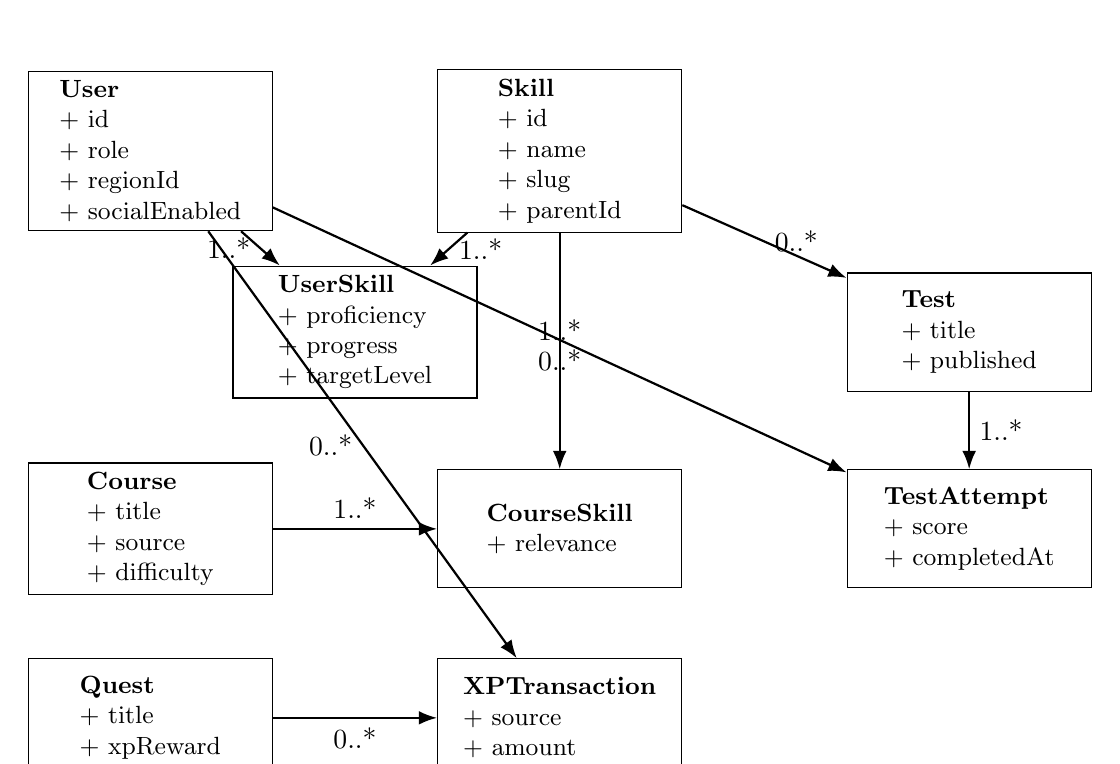
\begin{tikzpicture}[
  class/.style={draw, rectangle, minimum width=3.1cm, minimum height=1.5cm, align=left, font=\small},
  rel/.style={-Latex, thick}
]
\node[class] (user) at (0,0) {\textbf{User}\\+ id\\+ role\\+ regionId\\+ socialEnabled};
\node[class] (skill) at (5.2,0) {\textbf{Skill}\\+ id\\+ name\\+ slug\\+ parentId};
\node[class] (userskill) at (2.6,-2.3) {\textbf{UserSkill}\\+ proficiency\\+ progress\\+ targetLevel};
\node[class] (course) at (0,-4.8) {\textbf{Course}\\+ title\\+ source\\+ difficulty};
\node[class] (courseskill) at (5.2,-4.8) {\textbf{CourseSkill}\\+ relevance};
\node[class] (test) at (10.4,-2.3) {\textbf{Test}\\+ title\\+ published};
\node[class] (attempt) at (10.4,-4.8) {\textbf{TestAttempt}\\+ score\\+ completedAt};
\node[class] (quest) at (0,-7.2) {\textbf{Quest}\\+ title\\+ xpReward};
\node[class] (xp) at (5.2,-7.2) {\textbf{XPTransaction}\\+ source\\+ amount};

\draw[rel] (user) -- node[left] {1..*} (userskill);
\draw[rel] (skill) -- node[right] {1..*} (userskill);
\draw[rel] (course) -- node[above] {1..*} (courseskill);
\draw[rel] (skill) -- node[above] {1..*} (courseskill);
\draw[rel] (skill) -- node[right] {0..*} (test);
\draw[rel] (test) -- node[right] {1..*} (attempt);
\draw[rel] (user) -- node[below] {0..*} (attempt);
\draw[rel] (user) -- node[left] {0..*} (xp);
\draw[rel] (quest) -- node[below] {0..*} (xp);
\end{tikzpicture}
\caption{Zjednodušený diagram tříd/doménových entit systému SkillHub}
\label{fig:classdiagram}
\end{figure}

\section{Dokumentace API}
Protože projekt obsahuje vlastní backendové API, je jeho dokumentace povinnou součástí práce. Z důvodu přehlednosti je podrobný přehled jednotlivých endpointů, vstupních parametrů a vracených hodnot uveden v příloze A na straně \pageref{appendix-api}. Ve vlastní části práce je vhodné popsat spíše princip fungování API než opisovat dlouhé seznamy všech route.

\chapter{Výsledky}
\section{Dosažené moduly}
Výsledkem práce je funkční vícevrstvý systém, ve kterém byly implementovány hlavní moduly pro registraci a přihlášení, správu profilu, práci s dovednostmi, správu kurzů, testování, verifikaci, doporučování a volitelnou sociální vrstvu. Přehled stavu řešení shrnuje tab. \ref{tab:results}.

\begin{table}[ht]
\centering
\small
\caption{Přehled hlavních výstupů projektu}
\label{tab:results}
\begin{tabularx}{0.95\textwidth}{>{\raggedright\arraybackslash}p{3.2cm} >{\raggedright\arraybackslash}p{2.3cm} >{\raggedright\arraybackslash}X}
\toprule
Oblast & Stav & Stručný výsledek \\
\midrule
Autentizace a profil & implementováno & registrace, přihlášení, vazba na doménový profil, role a práce s osobními údaji \\
Dovednosti & implementováno & evidence skill profilu, úrovně, cílové úrovně a progresu \\
Kurzy a vazby na dovednosti & implementováno & kurzy propojené s dovednostmi pomocí relevance a zdrojového typu \\
Testování a verifikace & implementováno & běžné testy i samostatné ověření vyšších úrovní \\
Doporučování & implementováno & hybridní model s AI vrstvou a pravidlovým fallbackem \\
Social a gamifikace & implementováno & XP, questy, leaderboardy a opt-in režim \\
Administrace & částečně implementováno & správa uživatelů, dovedností, kurzů a questů \\
\bottomrule
\end{tabularx}
\normalsize
\end{table}

\section{Jak systém pracuje v praxi}
Po přihlášení uživatel vytvoří nebo doplní svůj profil dovedností. Backend kontroluje konzistenci vstupů a ukládá stav profilu do relační databáze. Změny v profilu následně ovlivňují doporučovací vrstvu i testovací logiku. Pokud uživatel chce zvýšit svou úroveň, systém mu nabídne test nebo verifikační pokus. V případě aktivovaného social režimu se navíc zapisují XP transakce a vyhodnocují questy.

Tento tok ukazuje, že jednotlivé části projektu nejsou izolované, ale tvoří provázaný celek. Právě tato provázanost je jedním z hlavních výsledků práce. Systém neslouží jen jako katalog nebo jen jako testovací modul, ale jako společná platforma pro plánování, studium, ověřování a motivaci.

\section{Důležité algoritmy}
Z pohledu implementace jsou nejdůležitější dva algoritmické principy. Prvním je výpočet relevance doporučení. Druhým je práce s gamifikačními body a vyhodnocování úrovně. Doporučení využívá sémantickou podobnost a zároveň bere v úvahu stav uživatelova skill profilu a relaci kurzu k dané dovednosti. Vztah lze vyjádřit například vzorcem:
\[
\mathrm{score}=\alpha \cdot \mathrm{sim}+\beta \cdot \mathrm{match}+\gamma \cdot \mathrm{relevance}
\]

Gamifikační vrstva naopak vychází z auditovatelných transakcí, takže každý bod XP má konkrétní zdroj a důvod zápisu. Tento princip je jednoduchý, ale důležitý pro kontrolu i budoucí rozšiřování systému.

\chapter{Diskuse}
\section{Zdůvodnění zvoleného řešení}
Zvolené řešení vychází z požadavku, aby projekt byl současně funkční, rozšiřitelný a přiměřený rozsahu maturitní práce. Z toho důvodu nebyl použit ani jednoduchý monolit bez oddělených vrstev, ani přehnaně složitá mikroservisní architektura. Zvolený model s frontendem, backendem a AI službou je dostatečně moderní, ale přitom stále provozně realistický.

Stejnou logiku sleduje i volba technologií. Frontendová část byla postavena na nástrojích, které jsou běžně používány při vývoji rozsáhlejších webových aplikací \cite{next,react}. Backendová část je záměrně jednodušší a přímočařejší, aby bylo možné dobře vysvětlit tok požadavků, middleware vrstvu i datový model \cite{express,prisma}. Autentizace byla svěřena specializované službě místo vlastní implementace, protože ta by přinášela zbytečné bezpečnostní riziko \cite{supabase,owasp}. AI část je oddělena, aby šlo v případě potřeby provozovat aplikaci i bez ní \cite{fastapi,reimers}.

\section{Výhody a limity projektu}
Hlavní výhodou projektu je provázání více funkcí do jednoho společného modelu. Uživatel nepracuje odděleně s katalogem kurzů, testovací službou a jinou aplikací pro motivaci, ale v jednom systému, který sdílí stejná data. Výhodou je také relativní otevřenost projektu. Protože jde o vlastní implementaci, lze systém upravovat podle konkrétních potřeb školy nebo jiného zadání.

Na druhé straně je nutné uvést i limity. Projekt nebyl testován na velkém množství reálných uživatelů, a proto nelze z této verze vyvozovat obecné závěry o dlouhodobé retenci nebo přesnosti doporučování v masovém provozu. Další limit spočívá v tom, že ne všechny administrační a instruktorské toky jsou dotaženy do stejně detailní podoby jako hlavní uživatelské scénáře.

\section{Ekonomické a provozní zhodnocení}
Pro studentský projekt je důležité, aby navržené řešení nebylo jen technicky zajímavé, ale také rozumné z pohledu provozu. SkillHub nevyžaduje nákladný cloudový model založený na permanentním volání velkých jazykových modelů. Využití lokální embeddingové vrstvy, cache a oddělených komponent zajišťuje rozumný kompromis mezi kvalitou výsledků, cenou a možností dalšího růstu.

Z provozního hlediska je důležitá i schopnost graceful degradation. Pokud AI služba selže, zbytek systému nepřestane fungovat, protože backend může přepnout na pravidlový fallback. Tato vlastnost je v praxi cennější než řešení, které má teoreticky nejvyšší přesnost, ale při chybě ztrácí funkčnost celého doporučování.

\chapter*{Závěr}
\addcontentsline{toc}{chapter}{Závěr}
Maturitní projekt SkillHub ukazuje, že i ve školním rozsahu lze navrhnout a implementovat systém, který nepůsobí jako izolované cvičení, ale jako smysluplný celek s reálnou přidanou hodnotou. Projekt propojuje práci s dovednostním profilem, doporučování, testování a motivaci do jedné architektury, kterou lze dále rozvíjet.

Dokumentace byla záměrně upravena tak, aby odpovídala školním pokynům: neobsahuje dlouhé marketingové výčty technologií, klade důraz na architekturu, postup řešení, výsledky a diskusi a doplňuje i povinnou API přílohu. Zároveň zůstává dostatečně stručná a věcná, což je pro kvalitní maturitní dokumentaci důležitější než formální objem textu bez skutečné informační hodnoty.

\clearpage
\addcontentsline{toc}{chapter}{Literatura}
\begin{thebibliography}{99}
\bibitem{next} VERCEL. \textit{Next.js Documentation} [online]. [cit. 2026-03-10]. Dostupné z: \url{https://nextjs.org/docs}
\bibitem{react} META. \textit{React Documentation} [online]. [cit. 2026-03-10]. Dostupné z: \url{https://react.dev/}
\bibitem{express} EXPRESS. \textit{Express.js Documentation} [online]. [cit. 2026-03-10]. Dostupné z: \url{https://expressjs.com/}
\bibitem{prisma} PRISMA. \textit{Prisma ORM Documentation} [online]. [cit. 2026-03-10]. Dostupné z: \url{https://www.prisma.io/docs}
\bibitem{supabase} SUPABASE. \textit{Supabase Documentation} [online]. [cit. 2026-03-10]. Dostupné z: \url{https://supabase.com/docs}
\bibitem{redis} REDIS LTD. \textit{Redis Documentation} [online]. [cit. 2026-03-10]. Dostupné z: \url{https://redis.io/docs/}
\bibitem{fastapi} FASTAPI. \textit{FastAPI Documentation} [online]. [cit. 2026-03-10]. Dostupné z: \url{https://fastapi.tiangolo.com/}
\bibitem{reimers} REIMERS, Nils a Iryna GUREVYCH. \textit{Sentence-BERT: Sentence Embeddings using Siamese BERT-Networks} [online]. arXiv:1908.10084. [cit. 2026-03-10]. Dostupné z: \url{https://arxiv.org/abs/1908.10084}
\bibitem{owasp} OWASP FOUNDATION. \textit{OWASP Top 10 Web Application Security Risks} [online]. [cit. 2026-03-10]. Dostupné z: \url{https://owasp.org/www-project-top-ten/}
\end{thebibliography}

\clearpage
\chapter*{Seznam obrázků, grafů a tabulek}
\addcontentsline{toc}{chapter}{Seznam obrázků, grafů a tabulek}
\listoffigures
\vspace{1cm}
\listoftables

\clearpage
\chapter*{Seznam příloh}
\addcontentsline{toc}{chapter}{Seznam příloh}
\begin{enumerate}
  \item Příloha A: Dokumentace API \dotfill \pageref{appendix-api}
\end{enumerate}

\clearpage
\pagenumbering{Roman}
\chapter*{Příloha A: Dokumentace API}
\label{appendix-api}
\addcontentsline{toc}{chapter}{Příloha A: Dokumentace API}
\scriptsize
\setlength{\tabcolsep}{3pt}
Následující přehled shrnuje hlavní endpointy backendového API. U každé položky je uvedena metoda, cesta, základní vstup a očekávaný výstup. Přehled je určen jako provozní a integrační dokumentace pro práci s aplikací.

\begin{longtable}{>{\raggedright\arraybackslash}p{1.15cm} >{\raggedright\arraybackslash}p{3.7cm} >{\raggedright\arraybackslash}p{4.1cm} >{\raggedright\arraybackslash}p{4.45cm}}
\caption{Hlavní endpointy backendového API}\\
\toprule
Metoda & Endpoint & Vstup & Návratová hodnota \\
\midrule
\endfirsthead
\toprule
Metoda & Endpoint & Vstup & Návratová hodnota \\
\midrule
\endhead
GET & \path{/api/health} & bez parametrů & stav služby, základní diagnostika \\
POST & \path{/api/auth/register} & e-mail, heslo, základní profilové údaje & vytvořený účet a navázaný uživatelský profil \\
POST & \path{/api/auth/login} & e-mail, heslo & access token, refresh token, uživatelská data \\
POST & \path{/api/auth/refresh} & refresh token & nová session a nové tokeny \\
POST & \path{/api/auth/logout} & platný token & potvrzení odhlášení \\
PATCH & \path{/api/auth/change-password} & currentPassword, newPassword & potvrzení změny hesla nebo nová session \\
POST & \path{/api/auth/oauth/initiate} & provider, redirectUrl & URL pro zahájení OAuth přihlášení \\
GET & \path{/api/auth/oauth/callback} & code, state & přihlášený uživatel a session po OAuth \\
POST & \path{/api/auth/complete-profile} & bearer token, jméno a profilové údaje & dokončení doménového profilu nebo chybový stav \\
GET & \path{/api/auth/me} & bearer token & detail aktuálně přihlášeného uživatele \\
GET & \path{/api/users/:id} & ID uživatele & veřejný profil a základní informace \\
GET & \path{/api/users/:id/profile} & bearer token, ID uživatele & plný profil uživatele včetně neveřejných polí \\
GET & \path{/api/users} & admin token, stránkování a filtry & stránkovaný seznam aktivních uživatelů \\
PATCH & \path{/api/users/:id} & bearer token, profilová data & aktualizovaný profil uživatele \\
POST & \path{/api/users/profile-picture} & obrázek multipart/form-data, bearer token & nové URL profilového obrázku a aktualizovaný profil \\
PATCH & \path{/api/users/:id/social-toggle} & bearer token, příznak social režimu & nový stav social režimu \\
GET & \path{/api/users/:id/stats} & bearer token nebo admin token & souhrn statistik studia, testů a bookmarků \\
GET & \path{/api/users/:id/activity} & bearer token nebo admin token, limit & poslední aktivita uživatele v systému \\
GET & \path{/api/users/:id/bookmarks} & bearer token, stránkování a řazení & seznam uložených bookmarků uživatele \\
POST & \path{/api/users} & courseId, bearer token & vytvořený bookmark kurzu pro přihlášeného uživatele \\
DELETE & \path{/api/users/:bookmarkId} & bearer token & odstranění bookmarku podle jeho ID \\
DELETE & \path{/api/users/course/:courseId} & bearer token & odstranění bookmarku podle ID kurzu \\
GET & \path{/api/users/:userId/skills} & ID uživatele & seznam uživatelských dovedností \\
POST & \path{/api/users/:userId/skills} & skillId, proficiency, progress, targetLevel & vytvořená vazba UserSkill \\
PATCH & \path{/api/users/:userId/skills/:skillId} & změna progress nebo proficiency & upravený záznam UserSkill \\
DELETE & \path{/api/users/:userId/skills/:skillId} & ID uživatele a skillu & potvrzení odstranění vazby \\
GET & \path{/api/users/:userId/skills/:skillId/progression} & bearer token & detail průběhu pro jednu dovednost \\
PATCH & \path{/api/users/:userId/skills} & dávkové úpravy profilu & aktualizovaný souhrn skill profilu \\
DELETE & \path{/api/users/:id} & bearer token nebo admin token & soft delete účtu uživatele \\
GET & \path{/api/users/deleted/list} & admin token, stránkování & seznam soft-deletovaných účtů \\
PATCH & \path{/api/users/:id/restore} & admin token & obnova smazaného účtu \\
POST & \path{/api/users/:id/clear-data} & bearer token & smazání studijních dat při zachování účtu \\
DELETE & \path{/api/users/:id/account} & bearer token & uživatelské zrušení vlastního účtu \\
GET & \path{/api/skills} & filtry, vyhledávání, parentId & seznam dovedností \\
GET & \path{/api/skills/:id} & ID dovednosti & detail dovednosti včetně vazeb \\
GET & \path{/api/skills/hierarchy/tree} & bez parametrů & strom dovedností od kořenových uzlů \\
GET & \path{/api/skills/search/advanced} & q, minUsers, hasCourses, hasTests atd. & rozšířené fulltextové vyhledání dovedností \\
GET & \path{/api/skills/categories} & bez parametrů & seznam dostupných kategorií dovedností \\
POST & \path{/api/skills} & bearer token, data dovednosti & vytvoření nové dovednosti \\
PATCH & \path{/api/skills/:id} & bearer token, změněná pole & aktualizace dovednosti \\
DELETE & \path{/api/skills/:id} & bearer token & odstranění dovednosti \\
GET & \path{/api/courses} & filtry jako skill, tag, difficulty, source & seznam kurzů se stránkováním \\
GET & \path{/api/courses/:id} & ID kurzu & detail kurzu, tagy, skill vazby a metadata \\
GET & \path{/api/courses/:id/lessons} & ID kurzu & seznam lekcí patřících ke kurzu \\
GET & \path{/api/courses/enrollments} & bearer token, stránkování & kurzy, do nichž je uživatel zapsán \\
GET & \path{/api/courses/:courseId/progress} & bearer token, ID kurzu & průběh studia v konkrétním kurzu \\
POST & \path{/api/courses} & bearer token, metadata kurzu & vytvoření interního kurzu \\
PATCH & \path{/api/courses/:id} & bearer token, změněná pole & aktualizace kurzu \\
DELETE & \path{/api/courses/:id} & bearer token & odstranění kurzu \\
POST & \path{/api/courses/:courseId/enroll} & bearer token & vytvoření enrollmentu uživatele \\
PATCH & \path{/api/courses/lessons/:lessonId/progress} & nový stav lekce & přepočet průběhu kurzu \\
POST & \path{/api/courses/import/youtube} & URL nebo metadata videa, bearer token & import kurzu z YouTube \\
POST & \path{/api/courses/generate-summaries} & bearer token, seznam kurzů & hromadně vygenerované AI souhrny \\
POST & \path{/api/courses/:id/generate-summary} & bearer token, ID kurzu & AI souhrn jednoho kurzu \\
GET & \path{/api/tests} & volitelné filtry & seznam testů \\
GET & \path{/api/tests/:id} & ID testu & detail testu včetně otázek a voleb \\
POST & \path{/api/tests} & admin token, definice testu & vytvoření nového testu \\
POST & \path{/api/tests/:id/attempts} & odpovídající token, ID testu & nový pokus o test \\
PATCH & \path{/api/tests/attempts/:attemptId} & odpovědi uživatele & průběžně nebo finálně vyhodnocený pokus \\
GET & \path{/api/tests/users/:id/attempts} & bearer token, ID uživatele & historie pokusů vybraného uživatele \\
GET & \path{/api/dashboard/stats} & admin token & agregační přehled hlavních entit a novinek \\
GET & \path{/api/stats} & bez autentizace & veřejné základní statistiky platformy \\
GET & \path{/api/recommendations} & bearer token, volba algoritmu & seznam doporučených kurzů nebo skillů \\
POST & \path{/api/recommendations/generate} & prompt nebo parametry uživatele & nově vygenerovaná doporučení \\
POST & \path{/api/recommendations/ai-skills} & textový prompt & doporučené dovednosti z AI vrstvy \\
GET & \path{/api/skills/:skillId/verification/questions} & ID dovednosti & sada verifikačních otázek \\
POST & \path{/api/skills/:skillId/verification/attempts} & odpovědi uživatele & nový verifikační pokus \\
PATCH & \path{/api/verification/attempts/:attemptId/submit} & dokončení pokusu & skóre, status pass/fail, doporučená úroveň \\
GET & \path{/api/verification/attempts/:attemptId} & bearer token, includeAnswers & detail jednoho verifikačního pokusu \\
GET & \path{/api/skills/:skillId/verification/attempts} & bearer token & seznam pokusů uživatele pro jednu dovednost \\
POST & \path{/api/verification/attempts/:attemptId/apply} & schválený výsledek & promítnutí verifikace do profilu uživatele \\
DELETE & \path{/api/verification/attempts/:attemptId} & bearer token & zrušení nedokončeného verifikačního pokusu \\
GET & \path{/api/skills/:skillId/verification/questions/admin} & admin token & kompletní sada verifikačních otázek pro správu \\
POST & \path{/api/skills/:skillId/verification/questions} & admin token, otázka a 4 volby & vytvoření nové verifikační otázky \\
PATCH & \path{/api/verification/questions/:questionId} & admin token, změněná pole a volby & aktualizace verifikační otázky \\
DELETE & \path{/api/verification/questions/:questionId} & admin token & odstranění verifikační otázky \\
POST & \path{/api/skills/:skillId/verification/questions/bulk} & admin token, pole otázek & dávkové založení verifikačních otázek \\
GET & \path{/api/verification/attempts/admin} & admin token, filtry a stránkování & přehled všech verifikačních pokusů \\
GET & \path{/api/social/profile} & bearer token & XP, level, streak a další social statistiky \\
GET & \path{/api/social/quests/daily} & bearer token & seznam denních questů a jejich stav \\
GET & \path{/api/social/leaderboard/weekly} & limit & veřejný týdenní leaderboard \\
GET & \path{/api/social/leaderboard/global} & limit & veřejný globální leaderboard \\
GET & \path{/api/social/xp/history} & bearer token & historie XP transakcí \\
POST & \path{/api/social/xp/award} & admin token, userId, amount, description & ruční přidání nebo odebrání XP \\
GET & \path{/api/social/quests/admin} & admin token & přehled všech questů \\
POST & \path{/api/social/quests} & admin token, definice questu & vytvořený quest \\
PATCH & \path{/api/social/quests/:id} & admin token, změněná pole & aktualizovaný quest \\
DELETE & \path{/api/social/quests/:id} & admin token & potvrzení odstranění questu \\
POST & \path{/api/social/quests/seed} & admin token & založení výchozích questů \\
GET & \path{/api/social/stats/quests} & admin token & agregované statistiky questů \\
GET & \path{/api/regions} & bez parametrů nebo s filtrem & seznam regionů \\
GET & \path{/api/regions/:id} & ID regionu & detail regionu včetně statistik a počtu uživatelů \\
GET & \path{/api/regions/:id/competition} & ID regionu, query skillId & data o regionální konkurenci pro jednu dovednost \\
GET & \path{/api/regions/:id/ranking/:userId} & bearer token & pořadí konkrétního uživatele v regionu \\
POST & \path{/api/regions} & bearer token, data regionu & vytvoření regionu \\
PATCH & \path{/api/regions/:id} & bearer token, změněná pole & aktualizace regionu \\
DELETE & \path{/api/regions/:id} & bearer token & odstranění regionu \\
GET & \path{/api/udemy/search} & query, page, pageSize a další filtry & výsledky vyhledání ve zdroji Udemy \\
GET & \path{/api/udemy/course/:courseId} & externí Udemy ID & detail externího kurzu \\
GET & \path{/api/udemy/imported} & page, limit, skillId & importované Udemy kurzy z interní DB \\
POST & \path{/api/udemy/admin/import} & externí ID kurzu, skill vazby & import kurzu do interní databáze \\
POST & \path{/api/udemy/admin/bulk-import} & query, maxCourses, skillIds & dávkový import výsledků vyhledávání \\
POST & \path{/api/udemy/admin/sync} & admin token & synchronizace již importovaných kurzů \\
GET & \path{/api/udemy/recommendations/:skillName} & bearer token, limit & doporučení externích kurzů podle skillu \\
GET & \path{/api/chapters/video/:videoId} & ID videa & detekované chapter značky a timestampy \\
POST & \path{/api/chapters/course/:courseId/update} & bearer token & aktualizace chapter značek jednoho kurzu \\
POST & \path{/api/chapters/batch-update} & bearer token, pole courseIds & dávková aktualizace více kurzů \\
POST & \path{/api/chapters/update-all-singles} & bearer token & zpracování všech kurzů s jedním videem \\
\bottomrule
\end{longtable}

\normalsize
\end{document}
